

\section{Approcci di classificazione}
\label{sec:approcci-di-classificazione}

Abbiamo diversi approcci di classificazione.

\begin{itemize}
    \item \textbf{Supervised learning}: Abbiamo un'insieme di dati che sono \textbf{etichettati}.
          Questo rappresenta il nostro \textbf{training set}. Il nostro obiettivo è fare
          predizioni sulle etichette di dati non ancora visti. Le etichette rappresentano
          la \textbf{classe}.
    \item \textbf{Unsupervised Learning}: I dati non hanno alcuna etichetta. Il nostro
          obiettivo è fare operazioni di \textbf{clustering}, ovvero raggruppare i dati in base a quanto sono simili tra loro.
    \item \textbf{Semisupervised Learning}: Abbiamo entrambi i tipi di dati (con e senza etichette). L'obiettivo è predirre la label
          dei dati non etichettati.
\end{itemize}

Il modo in cui chiamo i dati all'interno del nostro dataset sono molteplici,
tipo:
\begin{enumerate}
    \item Datum
    \item Object
    \item Feature Vectore / Vettore delle caratteristiche
    \item Punto
\end{enumerate}

\begin{definition}
    (Classifier)

    Un classificatore è una \textbf{superficie di separazione} tra le classi.
\end{definition}
\newpage
\section{Separazione Lineare}
\begin{definition}
    (Separazione Lineare)
    Dati due insiemi $A = \{a_1, a_2, \dots, \_m\}$ e $B = \{b_1, b_2, \dots, b_k\}$. Due insiemi si dicono \textbf{linearmente separabili} $\iff$ esiste un iperpiano $H(v,\gamma)$ che separa i due insiemi.

    $$
        H(v,\gamma) = \{x \in \mathcal{R}^n | v^T x = \gamma\}
    $$
    con:
    \begin{itemize}
        \item $v \in R^n$ è un vettore, la normale del piano
        \item $\gamma \in R$ è uno scalare, il bias
        \item $v \neq 0$
    \end{itemize}

    Questo iperpiano, tale che:

    $$
        v^T a_i \geq \gamma + 1 \land v^T b_j \leq \gamma - 1
    $$
    per $i = 1, \dots, m$ e $j = 1, \dots, k$.
\end{definition}

\textbf{Nota e possibile domanda}: Quando andiamo a classificare non teniamo conto del +1 e -1, perché vengono usati solo per costruzione.
Quindi la disequazione conta solamente il valore di $\gamma$ (nel lato desto).

\textbf{Nota 2:} I due insiemi $A$ e $B$ sono linearmente separabili $\iff$ \textbf{l'intersezione} della loro copertura convessa è vuota.
$$
    conv(A) \cap conv(B) = \emptyset
$$

\begin{definition}
    (Copertura Convessa)

    La copertura convessa di un'insieme $X$ è l'insieme convesso più piccolo che lo
    contiene.

    Un'insieme si dice convesso se per ogni coppia di punti $(x,y) \in X$ la
    combinazione di $x$ e $y$ è sempre all'interno dell'insieme $X$. Formalmente:
    $$ \forall x,y \in X, \forall \lambda \in [0,1] \implies \lambda x + (1 -
        \lambda) y \in X $$
\end{definition}

Implicazione ovvia, ma la copertura convessa di un'insieme convesso è l'insieme
stesso. $ X\ convesso \implies conv(X) = X $

\begin{definition}
    (Funzione Errore | Loss Function)

    Un punto $a_i \in A$ è \textbf{classificato correttamente} se $$ v^T a_i \geq
        \gamma + 1 \implies v^T a_i - \gamma - 1 \geq 0 $$ Questo implica che $a_i$ è
    \textbf{classificato erroneamente} se $$ v^T a_i - \gamma -1 < 0 \implies -v^T
        a_i + \gamma + 1 > 0 $$

    L'errore di $a_i$ è dato da: $$ \max\{0, -v^T a_i + \gamma + 1\} \geq 0 $$

    Analogamente, un punto $b_j \in B$ è \textbf{classificato correttamente} se $$
        v^T b_j - \gamma + 1 \leq 0 $$. Questo implica che $b_j$ è \textbf{classificato
        erroneamente} se $$ v^T b_j - \gamma + 1 > 0 $$

    L'errore di $b_j$ è dato da: $$ \max\{0, v^T b_j - \gamma + 1\} \geq 0 $$

    La funzione errore totale che ci viene da: $min_{v,\gamma} f(v,\gamma)$ è:

    $$
    \min_{v,\gamma} f(v,\gamma) = \frac{1}{m} \sum_{i=1}^{m} \max\{0, -v^T a_i + \gamma + 1\} + \frac{1}{k} \sum_{j=1}^{k} \max\{0, v^T b_j - \gamma + 1\}
    $$

    Cioè, la media degli errori di classificazione dei punti di $A$ e $B$.

    Questa funzioen è \textbf{non smooth e convessa}. Possiamo trasformare questo in un programma lineare.

    Consideriamo:
    \begin{itemize}
        \item $\xi  = \max{0, -v^T a_i + \gamma + 1}$ per $i = 1, \dots, m$
        \item $\psi_j = \max{0, v^T b_j - \gamma + 1}$ per $j = 1, \dots, k$
    \end{itemize}

    Possiamo riscrivere il problema nel seguente modo:

    $$
    LP = \begin{cases}
        \min_{v,\gamma, \xi, \psi} \frac{1}{m} \sum_{i=1}^{m} \xi_i + \frac{1}{k} \sum_{j=1}^{k} \psi_j \\

        \xi_i \geq -v^T a_i + \gamma + 1 \quad \forall i = 1, \dots, m \\
        \psi_j \geq v^T b_j - \gamma + 1 \quad \forall j = 1, \dots, k \\
        \xi_i, \psi_i \geq 0 \quad \forall i = 1\\
    \end{cases}
    $$
\end{definition}

\section{Separazione Poliedrale}
La separazione poliedrale è un'estensione della separazione lineare. In questo caso
consideriamo un problema che ha almeno $h > 1$ iperpiani di separazione $H(v^j, \gamma_j)$ tale che:
\begin{enumerate}
    \item Per ogni punto positivo $a_i \in A$ e ogni iperpiano $j = 1, \dots, h$ vale che:
    $$
        v^{jT} a_i \geq \gamma_j - 1
    $$

    Cioé il punto è "dentro" l'iperpiano.

    \item Per ogni punto negativo $b_i \in B$ esiste almeno 1 iperpiano $j \in \{1, \dots, h\}$ tale che:
    $$
        v^{jT} b_i \geq \gamma_j + 1
    $$

    Cioé il punto è "fuori" almeno 1 iperpiano.
\end{enumerate}

\textbf{Nota:} $A$ è h-pliedricamente separabile da $B$ $\iff$ $conv(A) \cap B = \emptyset$.

\textbf{Nota 2:} Se h = 1 $\rightarrow$ problema lineare.

\begin{definition}
    Funzione errore nel caso poliedrico:

    Un punto $a_i \in A$ è classificato correttamente se:

    $$
        v^{jT} a_i \leq \gamma_j -1 \quad \forall j = 1, \dots, h
    $$

    $$
        v^{jT} a_i - \gamma_j + 1 \leq 0 \quad \forall j = 1, \dots, h
    $$

    $$
        \max_{j=1, \dots, h} \{v^{jT} a_i - \gamma_j + 1\} \leq 0 \quad \forall j = 1, \dots, h
    $$

    Ed è classificato erroneamente se:

    $$
    \max_{j=1, \dots, h} \{v^{jT} a_i - \gamma_j + 1\} > 0 \quad \forall j = 1, \dots, h
    $$

    In totale, l'errore di $a_i$ è dato da:

    $$
        \max_{j=1, \dots, h} \{0, v^{jT} a_i - \gamma_j + 1\}
    $$

    Per quanto riguarda i punti negativi $b_j \in B$, viene classificato 
    correttamente se $\exists j \in \{1, \dots, h\}$ tale che:

    $$
    v^{jT} b_i \geq \gamma_j + 1 \rightarrow v^{jT} b_i - \gamma_j - 1 \geq 0 \rightarrow -v^{jT} b_i + \gamma_j + 1 \leq 0
    $$

    Analogamente, viene classificato erroneamente se:

    $$
    -v^{jT} b_i + \gamma_j + 1 > 0 \quad \forall j = 1, \dots, h
    $$

    Cioè, se $\min_{j=1, \dots, h} \{-v^{jT} b_i + \gamma_j + 1\} > 0$.

    L'errore di $b_i$ è dato da:

    $$
    \max_{j=1, \dots, h} \{0, -v^{jT} b_i + \gamma_j + 1\}
    $$    

    Notiamo che questa funzione è \textbf{più difficile da minimizzare}.

    \begin{figure}[H]
        \centering
        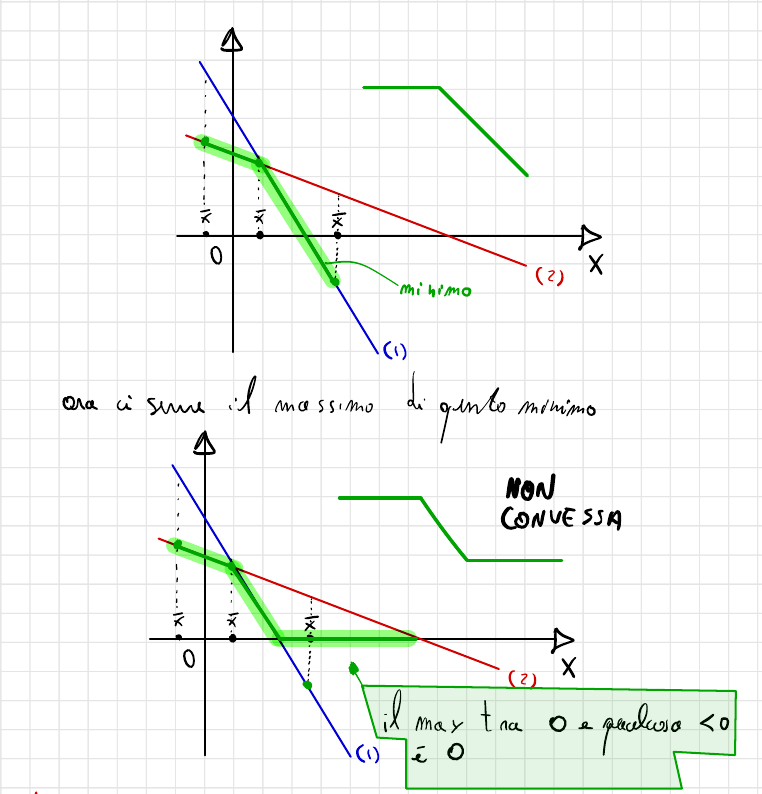
\includegraphics[width=0.8\linewidth]{images/tosta.png}
        \caption{Funzione di errore nel caso poliedrico}
        \label{fig:3-1}
    \end{figure}
    
    La funzione di errore 
    totale è data da:

    $$
        f ( v^1, v^2, \dots, v^; \gamma_1, \gamma_2, \dots, \gamma_h ) = \frac{1}{m} \sum_{i=1}^{m} \max_{j=1, \dots, h} \{0, v^{jT} a_i - \gamma_j + 1\} + \frac{1}{k} \sum_{j=1}^{k} \max_{j=1, \dots, h} \{0, -v^{jT} b_i + \gamma_j + 1\}
    $$

    Questa funzione è \textbf{non convessa}.
\end{definition}

